\documentclass{standalone}
\usepackage{tikz}
\begin{document}
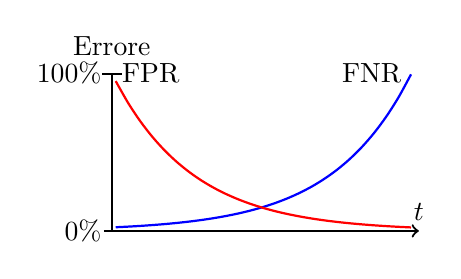
\begin{tikzpicture}
    \draw[thick, ->](-0.1,0)--++(4,0)node[above]{$t$};
    \draw[-|, thick](0,0)node[left]{$0\%$}--++(0,2.01)node[left]{$100\%$}node[right]{FPR};
    \draw[thick, blue]plot[smooth, domain=0.05:3.8](\x, {0.0445*e^(\x)});
    \draw[thick, red]plot[smooth, domain=0.05:3.8](\x, {2*e^(-\x)});
    \draw(3.8,2)node[left]{FNR};
    \draw(0,2.1)node[above]{Errore};
\end{tikzpicture}
\end{document}